\documentclass[degree=master]{thuthesis}
% 选项:
%   degree=[bachelor|master|doctor|postdoctor], % 必选
%   secret,                                     % 可选
%   pifootnote,                                 % 可选(建议打开)
%   openany|openright,                          % 可选,基本不用
%   arial,                                      % 可选,基本不用
%   arialtoc,                                   % 可选,基本不用
%   arialtitle                                  % 可选,基本不用

% 所有其它可能用到的包都统一放到这里了,可以根据自己的实际添加或者删除。
\usepackage{thuthesis}

% 定义所有的图片文件在 figures 子目录下
\graphicspath{{figures/}}

% 可以在这里修改配置文件中的定义。导言区可以使用中文。
% \def\myname{薛瑞尼}

\begin{document}

%%% 封面部分
\frontmatter
\thusetup{
  %******************************
  % 注意:
  %   1. 配置里面不要出现空行
  %   2. 不需要的配置信息可以删除
  %******************************
  %
  %=====
  % 秘级
  %=====
  secretlevel={公开},
  secretyear={2100},
  %
  %=========
  % 中文信息
  %=========
  ctitle={基于集中平台的RSCP-iBGP系统的研究与实现},
  %清华大学学位论文 \LaTeX\ 模板\\使用示例文档 v\version},
  cdegree={工学硕士},
  cdepartment={计算机科学与技术系},
  cmajor={计算机科学与技术},
  cauthor={王庆},
  csupervisor={尹霞教授},
  %cassosupervisor={陈文光教授}, % 副指导老师
  %ccosupervisor={某某某教授}, % 联合指导老师
  % 日期自动使用当前时间,若需指定按如下方式修改:
  % cdate={超新星纪元},
  %
  % 博士后专有部分
  cfirstdiscipline={计算机科学与技术},
  cseconddiscipline={系统结构},
  postdoctordate={2009年7月——2011年7月},
  id={编号}, % 可以留空: id={},
  udc={UDC}, % 可以留空
  catalognumber={分类号}, % 可以留空
  %
  %=========
  % 英文信息
  %=========
  etitle={A Study and Implement Based on Centralized Platform of RSCP-iBGP System},
  % 这块比较复杂,需要分情况讨论:
  % 1. 学术型硕士
  %    edegree:必须为Master of Arts或Master of Science(注意大小写)
  %             “哲学、文学、历史学、法学、教育学、艺术学门类,公共管理学科
  %              填写Master of Arts,其它填写Master of Science”
  %    emajor:“获得一级学科授权的学科填写一级学科名称,其它填写二级学科名称”
  % 2. 专业型硕士
  %    edegree:“填写专业学位英文名称全称”
  %    emajor:“工程硕士填写工程领域,其它专业学位不填写此项”
  % 3. 学术型博士
  %    edegree:Doctor of Philosophy(注意大小写)
  %    emajor:“获得一级学科授权的学科填写一级学科名称,其它填写二级学科名称”
  % 4. 专业型博士
  %    edegree:“填写专业学位英文名称全称”
  %    emajor:不填写此项
  edegree={Master of Science},
  emajor={Computer Science and Technology},
  eauthor={Wang Qing},
  esupervisor={Professor Yin Xia},
  %eassosupervisor={Chen Wenguang},
  % 日期自动生成,若需指定按如下方式修改:
  % edate={December, 2005}
  %
  % 关键词用“英文逗号”分割
   ckeywords={内部边界网关协议, 集中平台, 路由存储, 路由策略, 路由计算},
   ekeywords={Internal Border Gateway Protocol, Centralized Platform, Routing Storage, Routing Policy, Routing Calculation}
}


% 定义中英文摘要和关键字
\begin{cabstract}
  随着网络规模的不断扩大,自治系统内部需要逻辑全连接的内部边界网关协议iBGP,面临可扩展性问题。已有的研究方案路由反射、AS联邦、SoftRouter、RCP、RFCP等解决了iBGP的可扩展性,但带来了新的挑战。本文基于集中式体系结构的思路,提出基于集中平台的RSCP-iBGP系统,并充分利用集中平台的优势,在解决iBGP的可扩展问题的同时,也优化了路由存储和路由计算。如果自治系统内有N台边界路由器,iBGP全连接需要维护N平方的iBGP连接,路由表存储需要N份,在路由收敛的过程中路由计算需要最坏N平方次,而文中的新方案仅需维护N的iBGP连接,路由表存储O(1)份,路由表最坏计算N次。基于集中平台的RSCP-iBGP系统下,路由存储大小和路由计算次数均下降了一个数量级,该系统使得内部域间路由协议iBGP的性能、可扩展性提升很多。

  本文主要开展了以下工作:
  \begin{itemize}
    \item 针对iBGP可扩展问题,提出了基于集中平台的RSCP-iBGP系统,其中对路由存储、路由计算进行了优化,并将该系统与已有的5种方案进行对比分析,明确RSCP-iBGP系统相比于现有研究方案的优势。
    \item 设计RSCP-iBGP系统的工作流程、具体模块以及复式的最优路由计算算法,实现RSCP-iBGP系统中的三大模块:边界路由器,路由控制平台上的Route-Server,以及边界路由器与Route-Server之间的通信协议。
    \item 通过实验,对RSCP-iBGP系统进行功能验证。通过一致性测试工具PITSv3编写测试例对RSCP-iBGP系统进行功能一致性测试,最终验证了RSCP-iBGP系统的功能和设计相一致。
  \end{itemize}

\end{cabstract}

% 如果习惯关键字跟在摘要文字后面,可以用直接命令来设置,如下:
% \ckeywords{\TeX, \LaTeX, CJK, 模板, 论文}

\begin{eabstract}
   With the continuous expansion of network scale, internal border gateway protocol iBGP which requires a logical full mesh occurs scalability issue. Previous studies have solved the iBGP scalability issue, but brings new challenges, such as route reflection, AS federation, SoftRouter, RCP, RFCP, etc. This thesis proposes RSCP-iBGP system based on centralized platform to solve the iBGP scalability issue, which also optimizes routing storage and routing calculation. If there are N border routers in one Autonomous system, Full-Mesh IBGP needs to maintain N squared iBGP connections, to store N routing tables , and routing computing needs to execute N squared times in the process of routing convergence. RSCP-iBGP system only needs to maintain N iBGP connections, about one storage routing table, and routing computing needs to execute N times. The RSCP-iBGP system based on centralized platform contributes that size of routing storage and the number of routing computation are both reduced by an order of magnitude, And it improves the internal inter-domain routing protocols iBGP performance and scalability. The contributions of the work include:

   \begin{itemize}
    \item To solve scalability issue, the thesis puts forward the RSCP-iBGP system based on centralized platform, which optimizes routing storage and routing calculation. By comparing RSCP-iBGP system with and existing five schemes, the advantages of RSCP-iBGP system are confirmed.
    \item Design the work process, specific modules, multiple routing calculation algorithms, and RSCP-iBGP system realized three modules: border router, Route-Server running in the route control platform and the communication protocol.
    \item Execute functional verification of RSCP-iBGP system. The conformance testing of the RSCP-iBGP system was conducted by the conformance testing tool PITSv3, which finally verified that the realization of the RSCP-iBGP system is consistent with the design.
  \end{itemize}
\end{eabstract}




% \ekeywords{\TeX, \LaTeX, CJK, template, thesis}

% 如果使用授权说明扫描页,将可选参数中指定为扫描得到的 PDF 文件名,例如:
% \makecover[scan-auth.pdf]
\makecover

%% 目录
\tableofcontents

%% 符号对照表
\begin{denotation}[3cm]
\item[BGP] 边界网关协议(Border Gateway Protocol)
\item[iBGP] 内部边界网关协议 (Internal Border Gateway Protocol)
\item[eBGP] 外部边界网关协议 (External Border Gateway Protocol)
\item[EGP] 外部网关协议(Exterior Gateway Protocol)
\item[IGP] 内部网关协议(Interior Gateway Protocol)
\item[AS] 自治系统(Autonomous System)
\item[RR] 路由反射器(Router Reflector)
\item[RCP] 路由控制平台(Route Control Platform)
\item[RFCP] 路由流控制平台(Route Flow Control Platform)
\item[TCP] 传输控制协议(Transmission Control Protocol)
\item[MED] 多出口鉴别符(Multi-Exit Discriminators)
\item[SDN] 软件定义网络(Software-Defined Network)
\item[IXP] 网络交换节点(Internet Exchange Point)
\item[SDX] 软件定义的网络交换节点(Software Defined IXP)
\item[RSCP-iBGP] 基于路由控制平台的内部边界网关协议(Route Server Control Platform Internal Border Gateway Protocol)
\item[ASN] 自治系统号(Autonomous System Number)
\item[RIPv1] 路由信息协议版本1(Routing Information Protocol, Version 1)
\item[RIPv2] 路由信息协议版本2(Routing Information Protocol, Version 2)
\item[RIPng] 下一代路由信息协议(Routing Information Protocol, Next Generation)
\item[OSPFv2] 开放式最短路径优先版本2(Open Shortest Path First, Version 2)
\item[OSPFv3] 开放式最短路径优先版本3(Open Shortest Path First, Version 3)
\item[BGPv4+] 边界网关协议版本4扩展(Border Gateway Protocol, Version 4+)
\item[IS-IS] 中间系统到中间系统(Intermediate System-to-Intermediate System)
\item[PITSv3] 协议集成测试系统版本3(Protocol Integrated Test System, Version 3)
\end{denotation}



%%% 正文部分
\mainmatter
\chapter{引言}
\label{cha:intro}


\section{研究背景}

随着互联网的不断发展,自治系统的规模不断扩大,自治系统内的边界路由器数目和自治系统向外宣告前缀数目不断增加,互联网的域间路由协议面临多方面的挑战。边界网关协议(Border Gateway Protocol,BGP)是目前互联网使用的唯一的域间路由协议,直接影响网络功能和端到端的传输。早期设计BGP协议的阶段,自治系统(Autonomous System,AS)的数量和自治系统内部的边界路由器数量均较小,对BGP协议的可扩展性、安全性、路由策略的灵活性等缺乏关注。

BGP在AS内部所有路由器两两之间建立iBGP(Internal Border Gateway Protocol, iBGP)会话以交换域间路由,iBGP会话的数量是路由器平方数量级的,大型AS内部边界路由器的数目几百到上千,难以承受巨大的iBGP负担。学术界2000年左右提出了路由反射(Router Reflector, RR)和AS联邦的解决方案,两种方案虽然解决了全连接引起的可扩展性差的问题,但因为部分边界路由器缺少路由信息,带来了新的问题,比如非最优出口路由、转发环路、路由震荡等等,没有很好的解决当前网络环境下,iBGP面临的挑战。之后,有学者提出了基于集中式体系结构的SoftRouter、RCP(Route Control Platform)、RFCP(Route Flow Control Platform)等研究方案,在解决iBGP的可扩展问题的同时,保证所有边界路由器的路由决策基于全部的路由信息,解决了路由反射和AS联邦引发的新问题,同时该体系结构为路由存储、策略管理、路由计算提供了集中处理和管理的平台,使得内部域间路由具有很大的优化空间。

现有的基于集中式体系结构的iBGP研究,对路由存储、策略管理、路由计算的某些方面进行了优化,本文希望综合已有研究,在解决iBGP可扩展性的同时,将iBGP的路由存储、策略管理、路由计算的优化达到最大。

\section{主要工作}

本文对基于集中平台的RSCP-iBGP系统进行了实现、测试和评估,主要进行了以下工作:
\begin{enumerate}
\item 对BGP协议及其工作流程、域间路由协议iBGP存在的问题、以及解决iBGP存在问题的RR、AS联邦、SofterRouter、RCP、RFCP等研究方案、集中式思路优化BGP的相关研究进行了综述;
\item 介绍基于集中平台的RSCP-iBGP系统的整体框架,重点介绍路由存储和复式路由计算模块,并将该系统与现有的5种研究方案进行对比分析;
\item 对虚拟路由器Quagga的系统结构及路由更新等细节进行介绍,设计并实现基于集中平台的RSCP-iBGP系统;
\item 对RSCP-iBGP系统进行功能验证和系统评价实验,对RSCP-iBGP系统进行协议的一致性测试,验证RSCP-iBGP系统的功能一致性和性能优劣。
\end{enumerate}



\section{论文结构}
本文共包含六章:
\begin{itemize}
\item 第一章:引言,介绍研究背景和主要工作;
\item 第二章:相关研究综述,对BGP协议及工作流程、iBGP存在问题、iBGP可扩展性问题的研究现状、集中式思路优化BGP的相关研究等进行了综述;
\item 第三章:描述了基于集中平台的RSCP-iBGP系统的整体框架、系统模块,将其与已有方案进行对比分析;
\item 第四章:设计并实现基于集中平台的RSCP-iBGP系统,包括边界路由器、路由控制平台以及通信接口;
\item 第五章:对基于集中平台的RSCP-iBGP系统进行仿真实验和一致性测试,设计实验拓扑和一致性测试集,在实验床上运行扩展型iBGP协议,验证RSCP-iBGP系统的功能一致性和性能优劣;
\item 第六章:总结和进一步研究工作。
\end{itemize}

\chapter{中华人民共和国}
\label{cha:china}

\section{其它例子}
\label{sec:other}

在第~\ref{cha:intro} 章中我们学习了贝叶斯公式~(\ref{equ:chap1:bayes}),这里我们复
习一下:
\begin{equation}
\label{equ:chap2:bayes}
p(y|\mathbf{x}) = \frac{p(\mathbf{x},y)}{p(\mathbf{x})}=
\frac{p(\mathbf{x}|y)p(y)}{p(\mathbf{x})}
\end{equation}

\subsection{绘图}
\label{sec:draw}

本模板不再预先装载任何绘图包(如 \pkg{pstricks,pgf} 等),完全由用户来决定。
个人觉得 \pkg{pgf} 不错,不依赖于 Postscript。此外还有很多针对 \LaTeX{} 的
 GUI 作图工具,如 XFig(jFig), WinFig, Tpx, Ipe, Dia, Inkscape, LaTeXPiX,
jPicEdt, jaxdraw 等等。

\subsection{插图}
\label{sec:graphs}

强烈推荐《\LaTeXe\ 插图指南》!关于子图形的使用细节请参看 \pkg{subcaption} 宏包的说明文档。

\subsubsection{一个图形}
\label{sec:onefig}
一般图形都是处在浮动环境中。之所以称为浮动是指最终排版效果图形的位置不一定与源文
件中的位置对应\footnote{This is not a bug, but a feature of \LaTeX!},这也是刚使
用 \LaTeX{} 同学可能遇到的问题。如果要强制固定浮动图形的位置,请使用 \pkg{float} 宏包,
它提供了 \texttt{[H]} 参数,比如图~\ref{fig:xfig1}。
\begin{figure}[H] % use float package if you want it here
  \centering
  
\includegraphics{thu-whole-logo}
  \caption{利用 Xfig 制图}
  \label{fig:xfig1}
\end{figure}

大学之道,在明明德,在亲民,在止于至善。知止而后有定;定而后能静;静而后能安;安
而后能虑;虑而后能得。物有本末,事有终始。知所先后,则近道矣。古之欲明明德于天
下者,先治其国;欲治其国者,先齐其家;欲齐其家者,先修其身;欲修其身者,先正其心;
欲正其心者,先诚其意;欲诚其意者,先致其知;致知在格物。物格而后知至;知至而后
意诚;意诚而后心正;心正而后身 修;身修而后家齐;家齐而后国治;国治而后天下
平。自天子以至于庶人,壹是皆以修身为本。其本乱而未治者 否矣。其所厚者薄,而其所
薄者厚,未之有也!

\hfill —— 《大学》


\subsubsection{多个图形}
\label{sec:multifig}

如果多个图形相互独立,并不共用一个图形计数器,那么
用 \texttt{minipage} 或者\texttt{parbox} 就可以。否则,请参看
图~\ref{fig:big1-subcaptionbox},它包含两个小图,分别是图~\ref{fig:subfig1}和
图~\ref{fig:subfig2}。推荐使用 \cs{subcaptionbox},因为可以像
图~\ref{fig:big1-subcaptionbox} 那样对齐子图的标题,也可以使用 \pkg{subcaption}
宏包的 \cs{subcaption}(放在 minipage中,用法同\cs{caption})或
是 \pkg{subfigure} 、\pkg{subtable}环境,像图~\ref{fig:big1-subfigure},不要再
用 \cs{subfloat}、\cs{subfigure} 和 \cs{subtable}。

\begin{figure}[h]
  \centering%
  \subcaptionbox{第一个小图形\label{fig:subfig1}}[3cm] %标题的长度,超过则会换行,如下一个小图。
    {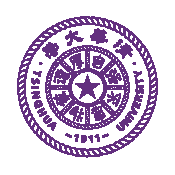
\includegraphics[height=3cm]{thu-fig-logo}}%
  \hspace{4em}%
  \subcaptionbox{第二个小图形,注意这个图略矮些。如果标题很长的话,它会自动换行\label{fig:subfig2}}
      {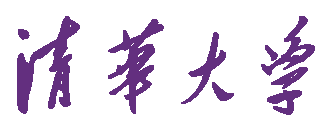
\includegraphics[height=2cm]{thu-text-logo}}
  \caption{包含子图形的大图形(subcaptionbox示例)}
  \label{fig:big1-subcaptionbox}
\end{figure}
\begin{figure}[h]
  \centering%
  \begin{subfigure}{3cm}
    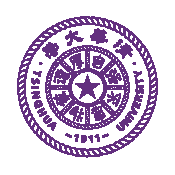
\includegraphics[height=3cm]{thu-fig-logo}
    \caption{第一个小图形}
  \end{subfigure}%
  \hspace{4em}%
  \begin{subfigure}{0.5\textwidth}
    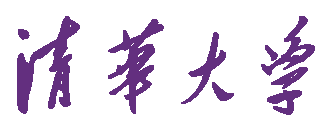
\includegraphics[height=2cm]{thu-text-logo}
    \caption{第二个小图形,注意这个图略矮些。subfigure中同一行的子图在顶端对齐。}
  \end{subfigure}
  \caption{包含子图形的大图形(subfigure示例)}
  \label{fig:big1-subfigure}
\end{figure}

古之学者必有师。师者,所以传道受业解惑也。人非生而知之者,孰能无惑?惑而不从师,
其为惑也,终不解矣。生乎吾前,其闻道也固先乎吾,吾从而师之;生乎吾後,其闻道也亦
先乎吾,吾从而师之。吾师道也,夫庸知其年之先後生於吾乎!是故无贵无贱无长无少,道
之所存,师之所存也。

嗟乎!师道之不传也久矣,欲人之无惑也难矣。古之圣人,其出人也远矣,犹且从师而问焉;
今之众人,其下圣人也亦远矣,而耻学於师。是故圣益圣,愚益愚。圣人之所以为圣,愚
人之所以为愚,其皆出於此乎?爱其子,择师而教之,於其身也,则耻师焉,惑焉。彼童子
之师,授之书而习其句读者,非吾所谓传其道、解其惑者也。句读之不知,惑之不解,或师
焉,或不焉,小学而大遗,吾未见其明也。巫医、乐师、百工之人不耻相师,  士大夫之族
曰“师”曰“弟子”之云者,则群聚而笑之。问之,则曰:彼与彼年相若也,道相似也,位
卑则足羞,官盛则近谀。呜呼!师道之不复,可知矣。巫医、乐师、百工之人。吾子不齿,
今其智乃反不能及,其可怪也欤!圣人无常师。孔子师郯子、苌子、师襄、老聃。郯子之徒,
其贤不及孔子。孔子曰:“三人行,必有我师。”是故弟子不必不如师,师不必贤於弟子。
闻道有先後,术业有专攻,如是而已。

如果要把编号的两个图形并排,那么小页就非常有用了:
\begin{figure}
\begin{minipage}{0.48\textwidth}
  \centering
  
\includegraphics[height=2cm]{thu-whole-logo}
  \caption{并排第一个图}
  \label{fig:parallel1}
\end{minipage}\hfill
\begin{minipage}{0.48\textwidth}
  \centering
  
\includegraphics[height=2cm]{thu-whole-logo}
  \caption{并排第二个图}
  \label{fig:parallel2}
\end{minipage}
\end{figure}

李氏子蟠,年十七,好古文、六艺,经传皆通习之,不拘於时,学於余。余嘉其能行古
道,作师说以贻之。

\hfill —— 韩愈(唐)



%%% 其它部分
\backmatter

%% 本科生要这几个索引,研究生不要。选择性留下。
% 插图索引
\listoffigures
% 表格索引
\listoftables
% 公式索引
\listofequations


%% 参考文献
% 注意:至少需要引用一篇参考文献,否则下面两行可能引起编译错误。
% 如果不需要参考文献,请将下面两行删除或注释掉。
% 数字式引用
\bibliographystyle{thuthesis-numeric}
% 作者-年份式引用
% \bibliographystyle{thuthesis-author-year}
\bibliography{ref/refs}


%% 致谢
% 如果使用声明扫描页,将可选参数指定为扫描后的 PDF 文件名,例如:
% \begin{acknowledgement}[scan-statement.pdf]
\begin{acknowledgement}
  衷心感谢导师尹霞教授,在我读硕士期间对我的关心和指导,并言传身教引导我树立严谨的科研态度和认真踏实的做事原则。在我科研长时间停滞不前的阶段,是尹霞老师的鼓励和支持,帮助我重拾科研的信心,语重心长地告诫我在科研上投入的时间不足,应“先做减法,再做加法”,让我迅速走出了科研困境。尹霞老师对实验室的同学都非常爱护,切身考虑同学们的处境和需要,关键时刻给我们很多精神上的大力支持和切合实际的宝贵建议,特别是在我毕业找工作的过程中,给予了我很多的帮助和建议。她不仅是我科研上的引领者,更是我人生的导师。

  万分感谢我的辅导老师王之梁老师,他批判性的科研思维和细致严谨的科研习惯,时时刻刻影响着我。硕士期间王老师一直悉心指导我的科研,定期与我讨论,明确指出我在科研上的一些陋习和思维缺陷,帮助我在科研上不断成长和进步。王老师在科研上对我的指导非常细致,有时我在实验阶段遇到瓶颈,王老师会亲自帮我查看并调试,我也能从中学习老师解决实际问题的方法,非常感激老师。以后在学习新东西的过程中,我也将继续保持在王老师教诲下养成的良好思维习惯及学习方式。

  非常感谢施新刚老师、姚姜源老师,他们对我在实验室的学习给了很大的帮助和支持。

  感谢实验室余家傲老师、张娜老师对我生活上的帮助,为实验室的同学创造了良好的科研环境。感谢实验室的张晗、郭迎亚、赵宗义、李亚慧、杨言、王苏、刘智峰、陈志鹏、马强、田莹等同学的帮助和鼓励,和他们的讨论帮助我解决了很多科研上的盲点,他们对我的鼓励促使我更加用心地投入到科研,感谢你们!


  %感谢 \LaTeX 和 \thuthesis\cite{thuthesis},帮我节省了不少时间。
\end{acknowledgement}


%% 附录
\begin{appendix}
\chapter{外文资料原文}
\label{cha:engorg}

\title{The title of the English paper}

\textbf{Abstract:} As one of the most widely used techniques in operations
research, \emph{ mathematical programming} is defined as a means of maximizing a
quantity known as \emph{bjective function}, subject to a set of constraints
represented by equations and inequalities. Some known subtopics of mathematical
programming are linear programming, nonlinear programming, multiobjective
programming, goal programming, dynamic programming, and multilevel
programming$^{[1]}$.

It is impossible to cover in a single chapter every concept of mathematical
programming. This chapter introduces only the basic concepts and techniques of
mathematical programming such that readers gain an understanding of them
throughout the book$^{[2,3]}$.


\section{Single-Objective Programming}
The general form of single-objective programming (SOP) is written
as follows,
\begin{equation}\tag*{(123)} % 如果附录中的公式不想让它出现在公式索引中,那就请
                             % 用 \tag*{xxxx}
\left\{\begin{array}{l}
\max \,\,f(x)\\[0.1 cm]
\mbox{subject to:} \\ [0.1 cm]
\qquad g_j(x)\le 0,\quad j=1,2,\cdots,p
\end{array}\right.
\end{equation}
which maximizes a real-valued function $f$ of
$x=(x_1,x_2,\cdots,x_n)$ subject to a set of constraints.

\newtheorem{mpdef}{Definition}[chapter]
\begin{mpdef}
In SOP, we call $x$ a decision vector, and
$x_1,x_2,\cdots,x_n$ decision variables. The function
$f$ is called the objective function. The set
\begin{equation}\tag*{(456)} % 这里同理,其它不再一一指定。
S=\left\{x\in\Re^n\bigm|g_j(x)\le 0,\,j=1,2,\cdots,p\right\}
\end{equation}
is called the feasible set. An element $x$ in $S$ is called a
feasible solution.
\end{mpdef}

\newtheorem{mpdefop}[mpdef]{Definition}
\begin{mpdefop}
A feasible solution $x^*$ is called the optimal
solution of SOP if and only if
\begin{equation}
f(x^*)\ge f(x)
\end{equation}
for any feasible solution $x$.
\end{mpdefop}

One of the outstanding contributions to mathematical programming was known as
the Kuhn-Tucker conditions\ref{eq:ktc}. In order to introduce them, let us give
some definitions. An inequality constraint $g_j(x)\le 0$ is said to be active at
a point $x^*$ if $g_j(x^*)=0$. A point $x^*$ satisfying $g_j(x^*)\le 0$ is said
to be regular if the gradient vectors $\nabla g_j(x)$ of all active constraints
are linearly independent.

Let $x^*$ be a regular point of the constraints of SOP and assume that all the
functions $f(x)$ and $g_j(x),j=1,2,\cdots,p$ are differentiable. If $x^*$ is a
local optimal solution, then there exist Lagrange multipliers
$\lambda_j,j=1,2,\cdots,p$ such that the following Kuhn-Tucker conditions hold,
\begin{equation}
\label{eq:ktc}
\left\{\begin{array}{l}
    \nabla f(x^*)-\sum\limits_{j=1}^p\lambda_j\nabla g_j(x^*)=0\\[0.3cm]
    \lambda_jg_j(x^*)=0,\quad j=1,2,\cdots,p\\[0.2cm]
    \lambda_j\ge 0,\quad j=1,2,\cdots,p.
\end{array}\right.
\end{equation}
If all the functions $f(x)$ and $g_j(x),j=1,2,\cdots,p$ are convex and
differentiable, and the point $x^*$ satisfies the Kuhn-Tucker conditions
(\ref{eq:ktc}), then it has been proved that the point $x^*$ is a global optimal
solution of SOP.

\subsection{Linear Programming}
\label{sec:lp}

If the functions $f(x),g_j(x),j=1,2,\cdots,p$ are all linear, then SOP is called
a {\em linear programming}.

The feasible set of linear is always convex. A point $x$ is called an extreme
point of convex set $S$ if $x\in S$ and $x$ cannot be expressed as a convex
combination of two points in $S$. It has been shown that the optimal solution to
linear programming corresponds to an extreme point of its feasible set provided
that the feasible set $S$ is bounded. This fact is the basis of the {\em simplex
  algorithm} which was developed by Dantzig as a very efficient method for
solving linear programming.
\begin{table}[ht]
\centering
  \centering
  \caption*{Table~1\hskip1em This is an example for manually numbered table, which
    would not appear in the list of tables}
  \label{tab:badtabular2}
  \begin{tabular}[c]{|m{1.5cm}|c|c|c|c|c|c|}\hline
    \multicolumn{2}{|c|}{Network Topology} & \# of nodes &
    \multicolumn{3}{c|}{\# of clients} & Server \\\hline
    GT-ITM & Waxman Transit-Stub & 600 &
    \multirow{2}{2em}{2\%}&
    \multirow{2}{2em}{10\%}&
    \multirow{2}{2em}{50\%}&
    \multirow{2}{1.2in}{Max. Connectivity}\\\cline{1-3}
    \multicolumn{2}{|c|}{Inet-2.1} & 6000 & & & &\\\hline
    \multirow{2}{1.5cm}{Xue} & Rui  & Ni &\multicolumn{4}{c|}{\multirow{2}*{\thuthesis}}\\\cline{2-3}
    & \multicolumn{2}{c|}{ABCDEF} &\multicolumn{4}{c|}{} \\\hline
\end{tabular}
\end{table}

Roughly speaking, the simplex algorithm examines only the extreme points of the
feasible set, rather than all feasible points. At first, the simplex algorithm
selects an extreme point as the initial point. The successive extreme point is
selected so as to improve the objective function value. The procedure is
repeated until no improvement in objective function value can be made. The last
extreme point is the optimal solution.

\subsection{Nonlinear Programming}

If at least one of the functions $f(x),g_j(x),j=1,2,\cdots,p$ is nonlinear, then
SOP is called a {\em nonlinear programming}.

A large number of classical optimization methods have been developed to treat
special-structural nonlinear programming based on the mathematical theory
concerned with analyzing the structure of problems.
\begin{figure}[h]
  \centering
  
\includegraphics{thu-lib-logo}
  \caption*{Figure~1\quad This is an example for manually numbered figure,
    which would not appear in the list of figures}
  \label{tab:badfigure2}
\end{figure}

Now we consider a nonlinear programming which is confronted solely with
maximizing a real-valued function with domain $\Re^n$.  Whether derivatives are
available or not, the usual strategy is first to select a point in $\Re^n$ which
is thought to be the most likely place where the maximum exists. If there is no
information available on which to base such a selection, a point is chosen at
random. From this first point an attempt is made to construct a sequence of
points, each of which yields an improved objective function value over its
predecessor. The next point to be added to the sequence is chosen by analyzing
the behavior of the function at the previous points. This construction continues
until some termination criterion is met. Methods based upon this strategy are
called {\em ascent methods}, which can be classified as {\em direct methods},
{\em gradient methods}, and {\em Hessian methods} according to the information
about the behavior of objective function $f$. Direct methods require only that
the function can be evaluated at each point. Gradient methods require the
evaluation of first derivatives of $f$. Hessian methods require the evaluation
of second derivatives. In fact, there is no superior method for all
problems. The efficiency of a method is very much dependent upon the objective
function.

\subsection{Integer Programming}

{\em Integer programming} is a special mathematical programming in which all of
the variables are assumed to be only integer values. When there are not only
integer variables but also conventional continuous variables, we call it {\em
  mixed integer programming}. If all the variables are assumed either 0 or 1,
then the problem is termed a {\em zero-one programming}. Although integer
programming can be solved by an {\em exhaustive enumeration} theoretically, it
is impractical to solve realistically sized integer programming problems. The
most successful algorithm so far found to solve integer programming is called
the {\em branch-and-bound enumeration} developed by Balas (1965) and Dakin
(1965). The other technique to integer programming is the {\em cutting plane
  method} developed by Gomory (1959).

\hfill\textit{Uncertain Programming\/}\quad(\textsl{BaoDing Liu, 2006.2})

\section*{References}
\noindent{\itshape NOTE: These references are only for demonstration. They are
  not real citations in the original text.}

\begin{translationbib}
\item Donald E. Knuth. The \TeX book. Addison-Wesley, 1984. ISBN: 0-201-13448-9
\item Paul W. Abrahams, Karl Berry and Kathryn A. Hargreaves. \TeX\ for the
  Impatient. Addison-Wesley, 1990. ISBN: 0-201-51375-7
\item David Salomon. The advanced \TeX book.  New York : Springer, 1995. ISBN:0-387-94556-3
\end{translationbib}

\chapter{外文资料的调研阅读报告或书面翻译}

\title{英文资料的中文标题}

{\heiti 摘要:} 本章为外文资料翻译内容。如果有摘要可以直接写上来,这部分好像没有
明确的规定。

\section{单目标规划}
北冥有鱼,其名为鲲。鲲之大,不知其几千里也。化而为鸟,其名为鹏。鹏之背,不知其几
千里也。怒而飞,其翼若垂天之云。是鸟也,海运则将徙于南冥。南冥者,天池也。
\begin{equation}\tag*{(123)}
 p(y|\mathbf{x}) = \frac{p(\mathbf{x},y)}{p(\mathbf{x})}=
\frac{p(\mathbf{x}|y)p(y)}{p(\mathbf{x})}
\end{equation}

吾生也有涯,而知也无涯。以有涯随无涯,殆已!已而为知者,殆而已矣!为善无近名,为
恶无近刑,缘督以为经,可以保身,可以全生,可以养亲,可以尽年。

\subsection{线性规划}
庖丁为文惠君解牛,手之所触,肩之所倚,足之所履,膝之所倚,砉然响然,奏刀騞然,莫
不中音,合于桑林之舞,乃中经首之会。
\begin{table}[ht]
\centering
  \centering
  \caption*{表~1\hskip1em 这是手动编号但不出现在索引中的一个表格例子}
  \label{tab:badtabular3}
  \begin{tabular}[c]{|m{1.5cm}|c|c|c|c|c|c|}\hline
    \multicolumn{2}{|c|}{Network Topology} & \# of nodes &
    \multicolumn{3}{c|}{\# of clients} & Server \\\hline
    GT-ITM & Waxman Transit-Stub & 600 &
    \multirow{2}{2em}{2\%}&
    \multirow{2}{2em}{10\%}&
    \multirow{2}{2em}{50\%}&
    \multirow{2}{1.2in}{Max. Connectivity}\\\cline{1-3}
    \multicolumn{2}{|c|}{Inet-2.1} & 6000 & & & &\\\hline
    \multirow{2}{1.5cm}{Xue} & Rui  & Ni &\multicolumn{4}{c|}{\multirow{2}*{\thuthesis}}\\\cline{2-3}
    & \multicolumn{2}{c|}{ABCDEF} &\multicolumn{4}{c|}{} \\\hline
\end{tabular}
\end{table}

文惠君曰:“嘻,善哉!技盖至此乎?”庖丁释刀对曰:“臣之所好者道也,进乎技矣。始臣之
解牛之时,所见无非全牛者;三年之后,未尝见全牛也;方今之时,臣以神遇而不以目视,
官知止而神欲行。依乎天理,批大郤,导大窾,因其固然。技经肯綮之未尝,而况大坬乎!
良庖岁更刀,割也;族庖月更刀,折也;今臣之刀十九年矣,所解数千牛矣,而刀刃若新发
于硎。彼节者有间而刀刃者无厚,以无厚入有间,恢恢乎其于游刃必有余地矣。是以十九年
而刀刃若新发于硎。虽然,每至于族,吾见其难为,怵然为戒,视为止,行为迟,动刀甚微,
謋然已解,如土委地。提刀而立,为之而四顾,为之踌躇满志,善刀而藏之。”

文惠君曰:“善哉!吾闻庖丁之言,得养生焉。”


\subsection{非线性规划}
孔子与柳下季为友,柳下季之弟名曰盗跖。盗跖从卒九千人,横行天下,侵暴诸侯。穴室枢
户,驱人牛马,取人妇女。贪得忘亲,不顾父母兄弟,不祭先祖。所过之邑,大国守城,小
国入保,万民苦之。孔子谓柳下季曰:“夫为人父者,必能诏其子;为人兄者,必能教其弟。
若父不能诏其子,兄不能教其弟,则无贵父子兄弟之亲矣。今先生,世之才士也,弟为盗
跖,为天下害,而弗能教也,丘窃为先生羞之。丘请为先生往说之。”
\begin{figure}[h]
  \centering
  
\includegraphics{thu-whole-logo}
  \caption*{图~1\hskip1em 这是手动编号但不出现索引中的图片的例子}
  \label{tab:badfigure3}
\end{figure}

柳下季曰:“先生言为人父者必能诏其子,为人兄者必能教其弟,若子不听父之诏,弟不受
兄之教,虽今先生之辩,将奈之何哉?且跖之为人也,心如涌泉,意如飘风,强足以距敌,
辩足以饰非。顺其心则喜,逆其心则怒,易辱人以言。先生必无往。”

孔子不听,颜回为驭,子贡为右,往见盗跖。

\subsection{整数规划}
盗跖乃方休卒徒大山之阳,脍人肝而餔之。孔子下车而前,见谒者曰:“鲁人孔丘,闻将军
高义,敬再拜谒者。”谒者入通。盗跖闻之大怒,目如明星,发上指冠,曰:“此夫鲁国之
巧伪人孔丘非邪?为我告之:尔作言造语,妄称文、武,冠枝木之冠,带死牛之胁,多辞缪
说,不耕而食,不织而衣,摇唇鼓舌,擅生是非,以迷天下之主,使天下学士不反其本,妄
作孝弟,而侥幸于封侯富贵者也。子之罪大极重,疾走归!不然,我将以子肝益昼餔之膳。”


\chapter{其它附录}
前面两个附录主要是给本科生做例子。其它附录的内容可以放到这里,当然如果你愿意,可
以把这部分也放到独立的文件中,然后将其 \cs{input} 到主文件中。

\end{appendix}

%% 个人简历
\begin{resume}

  \resumeitem{个人简历}

  xxxx 年 xx 月 xx 日出生于 xx 省 xx 县。

  xxxx 年 9 月考入 xx 大学 xx 系 xx 专业,xxxx 年 7 月本科毕业并获得 xx 学士学位。

  xxxx 年 9 月免试进入 xx 大学 xx 系攻读 xx 学位至今。

  \researchitem{发表的学术论文} % 发表的和录用的合在一起

  % 1. 已经刊载的学术论文(本人是第一作者,或者导师为第一作者本人是第二作者)
  \begin{publications}
    \item Yang Y, Ren T L, Zhang L T, et al. Miniature microphone with silicon-
      based ferroelectric thin films. Integrated Ferroelectrics, 2003,
      52:229-235. (SCI 收录, 检索号:758FZ.)
    \item 杨轶, 张宁欣, 任天令, 等. 硅基铁电微声学器件中薄膜残余应力的研究. 中国机
      械工程, 2005, 16(14):1289-1291. (EI 收录, 检索号:0534931 2907.)
    \item 杨轶, 张宁欣, 任天令, 等. 集成铁电器件中的关键工艺研究. 仪器仪表学报,
      2003, 24(S4):192-193. (EI 源刊.)
  \end{publications}

  % 2. 尚未刊载,但已经接到正式录用函的学术论文(本人为第一作者,或者
  %    导师为第一作者本人是第二作者)。
  \begin{publications}[before=\publicationskip,after=\publicationskip]
    \item Yang Y, Ren T L, Zhu Y P, et al. PMUTs for handwriting recognition. In
      press. (已被 Integrated Ferroelectrics 录用. SCI 源刊.)
  \end{publications}

  % 3. 其他学术论文。可列出除上述两种情况以外的其他学术论文,但必须是
  %    已经刊载或者收到正式录用函的论文。
  \begin{publications}
    \item Wu X M, Yang Y, Cai J, et al. Measurements of ferroelectric MEMS
      microphones. Integrated Ferroelectrics, 2005, 69:417-429. (SCI 收录, 检索号
      :896KM)
    \item 贾泽, 杨轶, 陈兢, 等. 用于压电和电容微麦克风的体硅腐蚀相关研究. 压电与声
      光, 2006, 28(1):117-119. (EI 收录, 检索号:06129773469)
    \item 伍晓明, 杨轶, 张宁欣, 等. 基于MEMS技术的集成铁电硅微麦克风. 中国集成电路,
      2003, 53:59-61.
  \end{publications}

  \researchitem{研究成果} % 有就写,没有就删除
  \begin{achievements}
    \item 任天令, 杨轶, 朱一平, 等. 硅基铁电微声学传感器畴极化区域控制和电极连接的
      方法: 中国, CN1602118A. (中国专利公开号)
    \item Ren T L, Yang Y, Zhu Y P, et al. Piezoelectric micro acoustic sensor
      based on ferroelectric materials: USA, No.11/215, 102. (美国发明专利申请号)
  \end{achievements}

\end{resume}


%% 本科生进行格式审查是需要下面这个表格,答辩可能不需要。选择性留下。
% 综合论文训练记录表
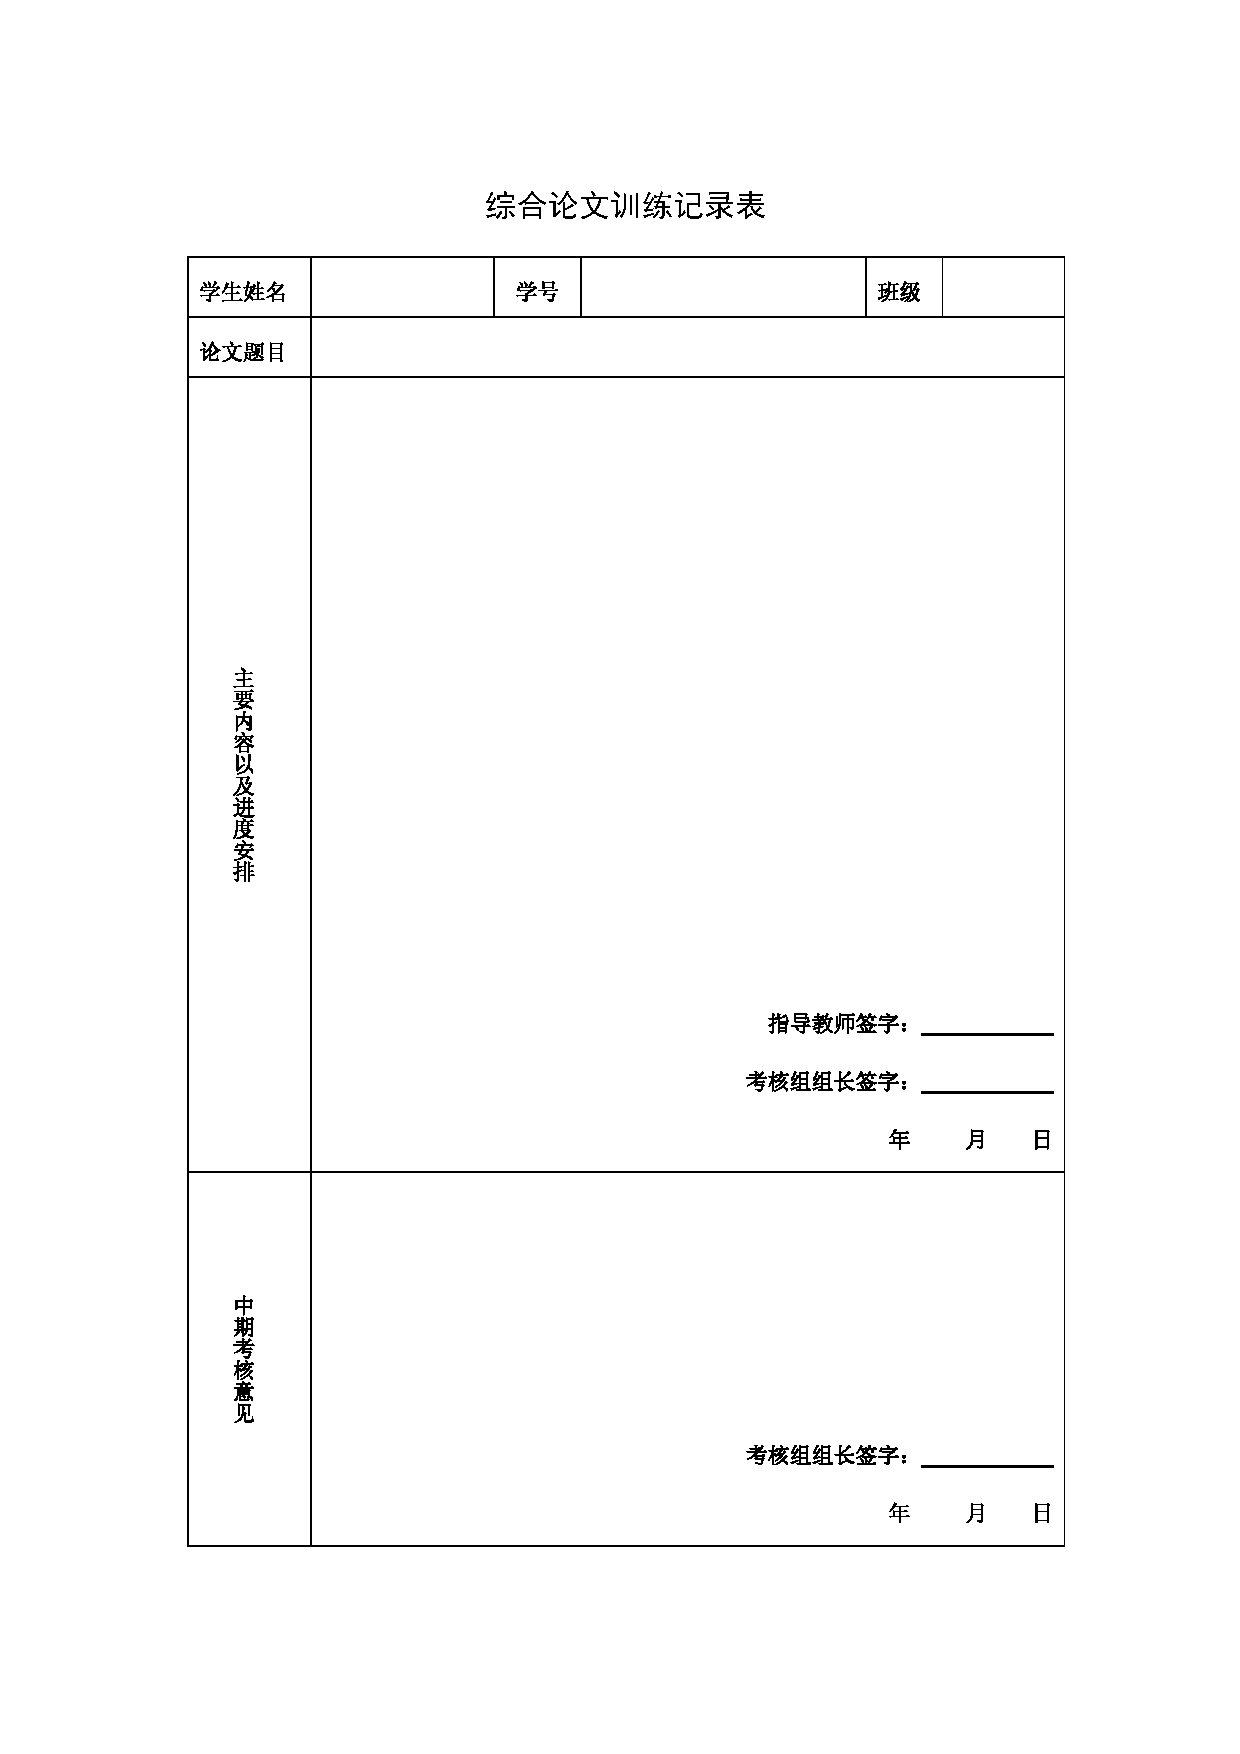
\includepdf[pages=-]{scan-record.pdf}
\end{document}
